\documentclass[12pt]{article}
\usepackage{color}
\usepackage[usenames,dvipsnames,svgnames,table]{xcolor}
\definecolor{dark-red}{rgb}{0.7,0.1,0.1} 
\definecolor{dark-blue}{rgb}{0,0,0.7} 
\usepackage[linkcolor=dark-red,
            colorlinks=true,
            urlcolor=dark-blue,
            pdfstartview={XYZ null null 1.00},
            pdfauthor={Gaurav Sood, gsood07@gmail.com},
            citecolor=dark-red,
            bookmarks=false,
            pdfborder={0 0 0},
            pdftitle={The Review}]{hyperref}
            
\usepackage{amsfonts,amssymb,amsbsy,amsmath,amsxtra}

\usepackage[letterspace=1000]{microtype}
\usepackage{libertine}
\usepackage[T1]{fontenc}

\usepackage{indentfirst}
\usepackage{setspace} % To set line spacing
\usepackage{multirow}

\usepackage{verbatim}

\usepackage[multiple]{footmisc}
\usepackage{fancyvrb}

\usepackage{longtable}

\usepackage[margin=1in]{geometry}
\usepackage{graphicx}

\raggedright
\parindent=1.5em % <- or whatever indent you want

\usepackage{natbib}
\usepackage{url}
\begin{comment}

setwd(paste0(githubdir, "/meta_apsr/ms/"))	
tools::texi2dvi("the_review.tex", pdf=TRUE, clean=TRUE)	
setwd(paste0(githubdir, "/meta_apsr/"))

\end{comment}

\begin{document}
\title{\vspace{-.5cm}\normalsize{The Review: Production and Consumption of APSR\footnote{The data, and the scripts to acquire, process and analyze the data can be found at \href{https://github.com/soodoku/meta_apsr}{https://github.com/soodoku/meta\_apsr}.}
}}
\author{\vspace{.2cm}\\\normalsize{Gaurav Sood}\\\href{mailto:gsood07@gmail.com}{\small{gsood07@gmail.com}}\vspace{.3cm}\\}
\date{\normalsize{November 20th, 2015}}
\maketitle
\begin{center}
\textbf{NB:} Preliminary draft. Please do not cite without permission.
\end{center}
\vspace{.4cm}
\doublespacing

Scientific production is affected by a variety of variables that have little to do with science. For instance, investment in research is correlated with commercialization lags--- greater the lags, lower the investment \citep{budish2013firms}.\footnote{The article posits that later stage cancer drugs have smaller commercialization lags. It isn't clear why. But the general point likely holds.} On the flip side, minor changes in how the research is delivered can have large effects on consumption of research. For instance, papers listed first in National Bureau of Economic Research email digests get 27\% more citations than papers listed at other locations.\footnote{ See \href{http://www.npr.org/2015/07/15/423101360/no-1-with-a-bullet-point-to-get-research-cited-make-sure-its-listed-first}{http://www.npr.org/2015/07/15/423101360/no-1-with-a-bullet-point-to-get-research-cited-make-sure-its-listed-first}.} More generally, a broad range of factors, from availability of funding to fads to various parts of the scientific paper production pipeline, including, the number of articles editors must review, the incentives to be nice to the author, likely affect what topic is researched, the quality of the research, who produces the research, and how many read it. 

Using an original dataset of rich meta data on all articles published in the The American Political Science Review (APSR), the preeminent political science journal, I shed light on some of these issues. In particular, I study whether, like top economic journals, over time the number of articles published by The Review has declined \citep{card2013nine, card2014page}. I find that the number of articles published by the APSR has increased over time, though the number of articles per issue has plateaued over the last thirty or so years.

Next, I investigate two particular aspects of production: co-authorship and gender of authors. For a variety of reasons--- ease of co-authorship, greater differentiation in skills, greater complexity of projects--- the proportion of co-authored articles in a variety of fields is on the rise \citep{barnett1988rising, card2013nine, cunningham1997authorship}. I study whether that is true for the APSR. Expectedly, I find that co-authorship rates have increased significantly. Second, I estimate the proportion of women per published article in the APSR over time. While the proportion has increased over time, it still remains very low.  

Next, I move to study consumption using consumption. I find that both the abstract views and full-text views follow the well-known power law distribution, with a few articles receiving a lot of views and most articles receiving no views. I end by investigating something fun. Some previous analyses have suggested that paper titles have gotten longer over time.\footnote{See \href{http://datacolada.org/2013/12/04/titleogy/}{http://datacolada.org/2013/12/04/titleogy/}} I check whether this is true for the APSR. I find that it is.

\section*{Data and Results} 
I scrape the APSR website for the data. Scraping yields a dataset of 30,235 unique document objects. These documents include editor's notes, rejoinders, articles, research notes, book reviews and other miscellanea that have been published in the APSR. I exclude editor's notes, book reviews, etc. from the data. This leaves us with 4,385 articles, which serves as the final dataset. For each article, we know the title, the abstract and the pages spanned (though not the font or the line spacing or the page margins), the names and institutional affiliations of the authors, and the total number of times the abstract, and the full-text of the article have been viewed. In addition, we have information on the number of pages in each issue (volume). To these data, I add imputed gender of the authors --- proportion of people with the name who were female according to the census--- using the {\tt R} Package {\tt gender} \citep{lincoln2015}.\footnote{There are at least two major limitations in how the gender of the names is imputed. First, time can be correlated with gender distribution of a name, and we lack information on the age of the author. I assume that the age of an author's age is uniformly distributed between 25 and 65. While this is unsatisfactory, using different ranges yields very similar results. Second, the data on the names is only from the U.S. Expanding the database to include data from Canada and Europe are obvious next steps.} I use these data to answer the questions.

The number of articles published in the top economics journal, The American Economic Review (AER), has declined over the years \citep{card2014page}.\footnote{The Quarterly Journal of Economics is the top-ranked economics journal by some measures today.} This surprising pattern is a result of longer articles and constant size of the issue \citep{card2014page}.\footnote{\citet{ellison2000evolving} humorously notes, ``Ariel Rubinstein's 1982 Econometrica article, `Perfect Equilibrium in a Bargaining Model,' for example, is about as long as the average note in Econometrica in 2001.''} (Over the past few years, the AER has capped article length.) To see whether the same holds for The APSR, I first investigate article length. Over the past 100 or so years, average article length has shown marked variability (see Figure~\ref{fig:pages}). But unlike top economics journals there is no trend towards longer articles. (It is very likely, however, that the length of online appendices has grown substantially.) This likely reflects a longer tradition of capping article lengths in political science.

Moving to number of articles per issue, unlike top economic journals, over the last hundred years, the number of articles per issue has more than doubled (see Figure~\ref{fig:narticles}). Though, over the past thirty or so years, the number of articles per issue has plateaued. Given no trend in article length, and increase in number of articles per issue, it has to be that pages per issue would have increased. And so we find (see Figure~\ref{fig:issue}). 

Next, we analyze data on two aspects of production: number of authors per article, and proportion of female authors per article. Looking at the number of authors per article over time, like in other places, co-authorship is on the rise. Though, solo authored papers still make a sizable proportion of publications in the APSR, the modal publication today has two authors (see Figure~\ref{fig:nauthors}). As for proportion of women per article, the data are distressing. While the proportion of women on each article published in the APSR has risen consistently and sharply, the average article still has just 20\% female authors (see Figure~\ref{fig:women}). (Pairing it with American Political Science Association membership data would provide one (still unsatisfactory) way of getting an estimate of gender bias.)

Flipping the lens and looking at two consumption metrics: number of abstract views and number of full-text views, provides a familiar power-law distribution. Most of the articles (abstracts) aren't viewed at all. And a small set of articles gets a lot of views (see Figures~\ref{fig:abstracts} and ~\ref{fig:fulltext}).

Lastly, some fun. Plotting the length of titles of APSR articles over time clearly shows that the titles have become longer over time. In fact, the average title length has increased by 50\%--- from an average of 50 to about 75 characters today.

\clearpage
\begin{center}
\large{Figures}
\end{center}

\begin{figure}[htbp]
\centering
\caption{Number of Pages per Article Over Time}
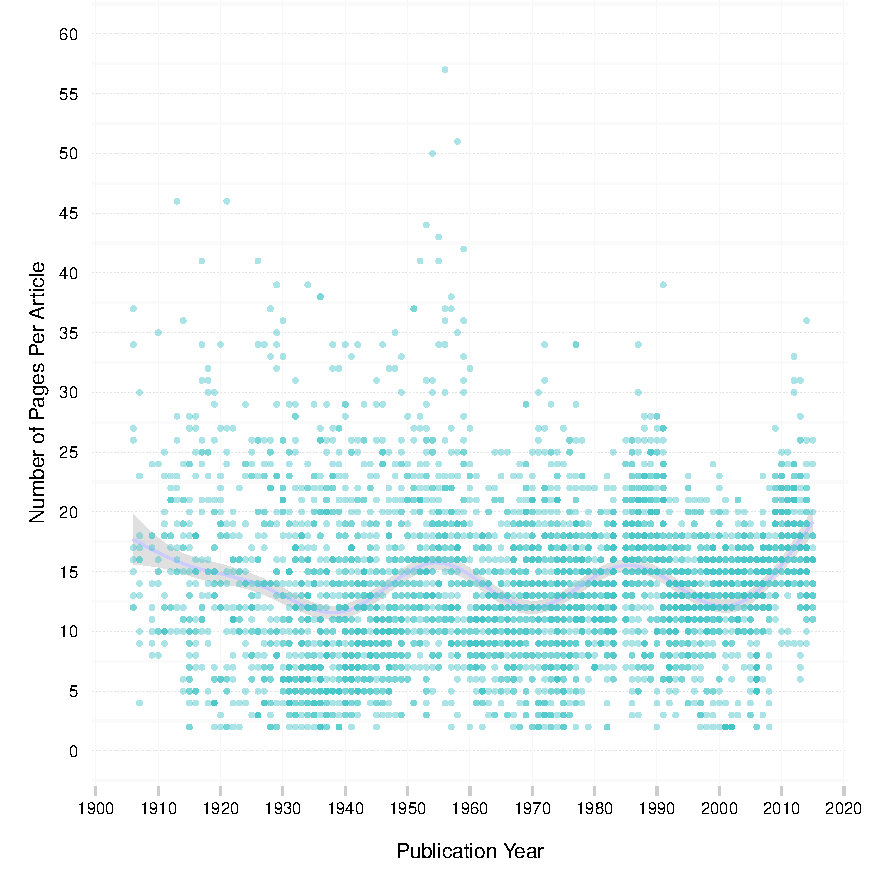
\includegraphics[scale=.85]{../figs/n_pages_per_article_over_time.pdf}
\label{fig:pages}
\end{figure}

\begin{figure}[htbp]
\centering
\caption{Number of Articles per Issue Over Time}
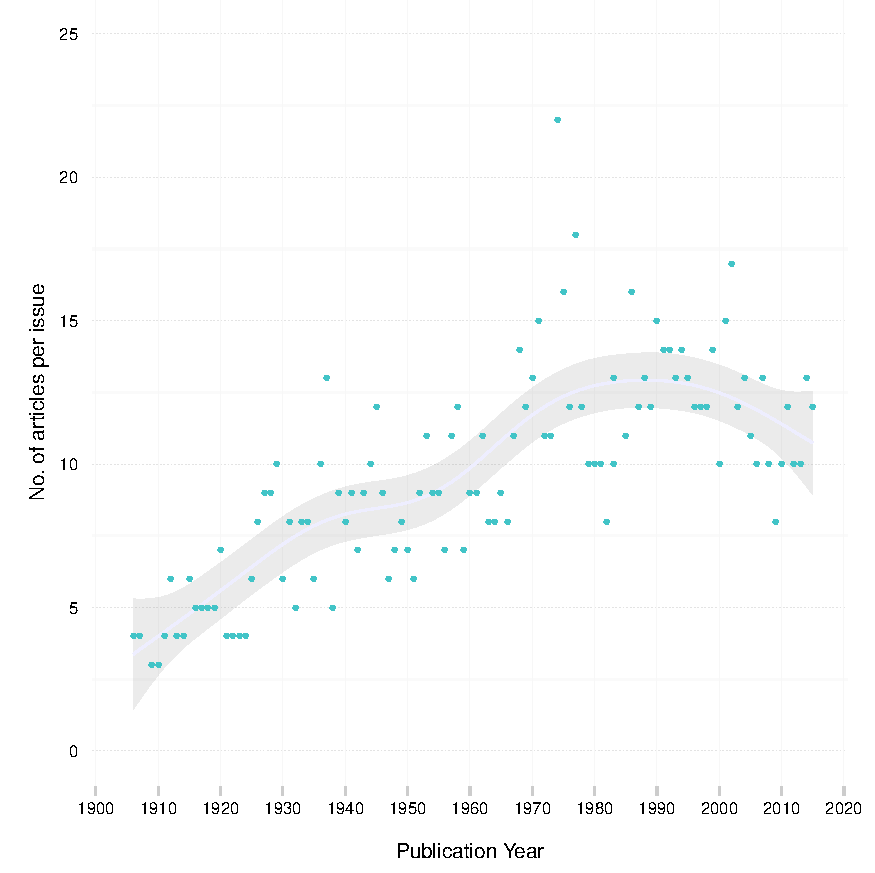
\includegraphics[scale=.85]{../figs/articles_per_issue_over_time.pdf}
\label{fig:narticles}
\end{figure}

\begin{figure}[htbp]
\centering
\caption{Pages per Issue Over time}
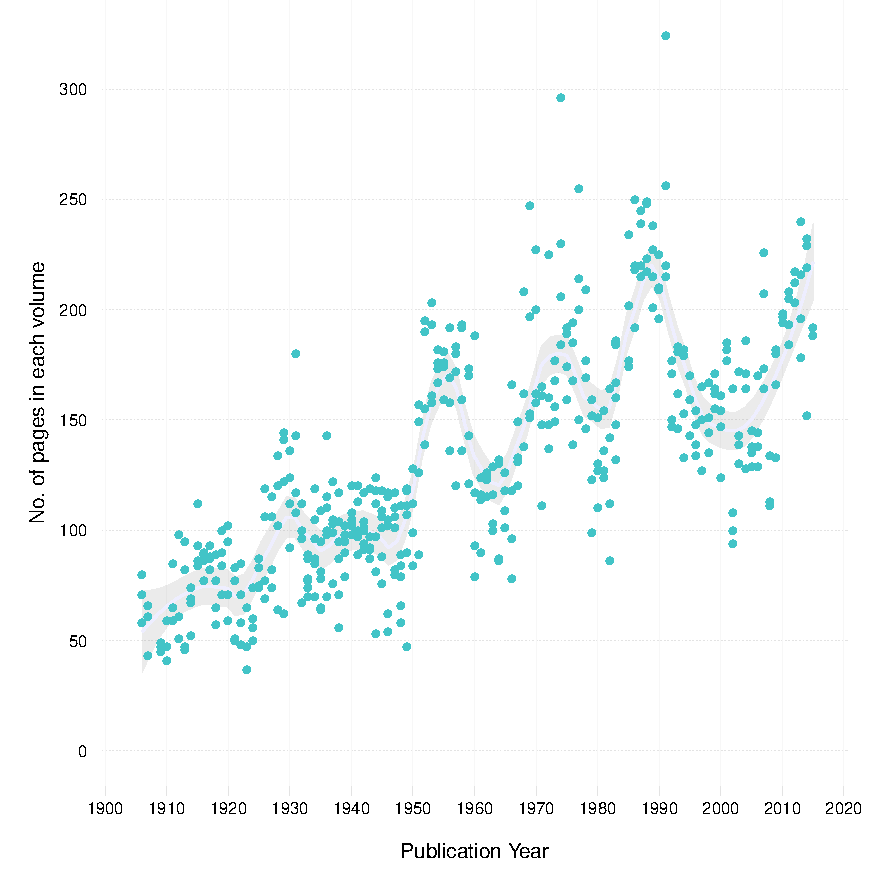
\includegraphics[scale=.85]{../figs/pages_per_issue_over_time.pdf}
\label{fig:issue}
\end{figure}

\begin{figure}[htbp]
\centering
\caption{Number of Authors per Article Over Time}
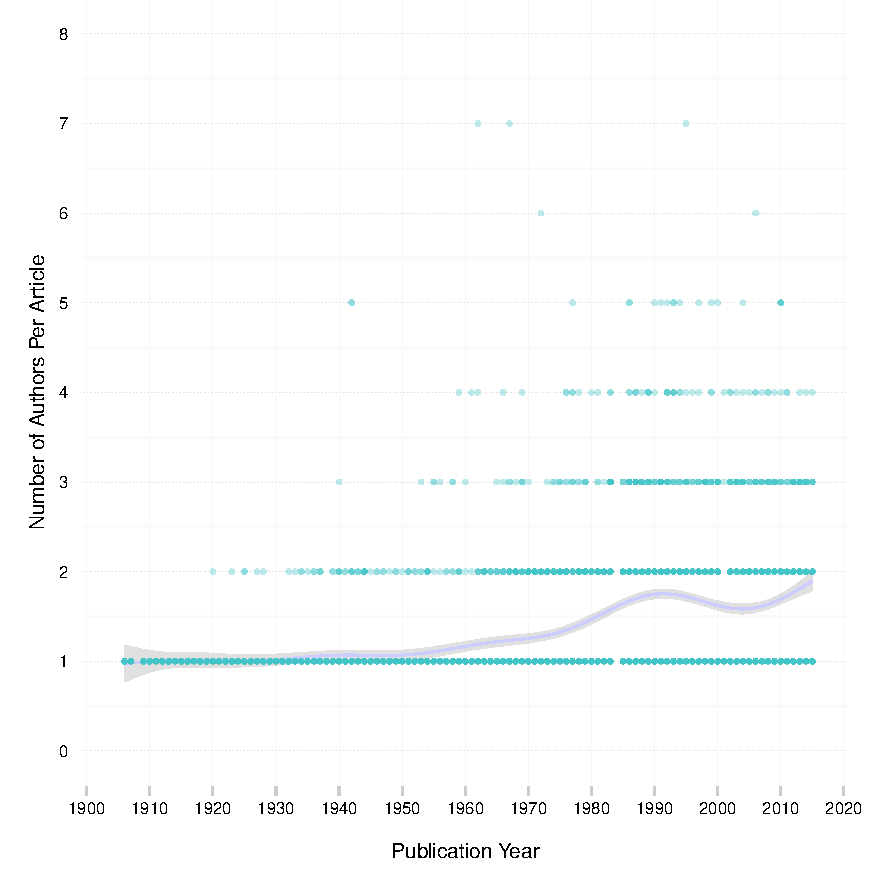
\includegraphics[scale=.85]{../figs/n_authors_per_article_over_time.pdf}
\label{fig:nauthors}
\end{figure}

\begin{figure}[htbp]
\centering
\caption{Proportion of Women Per Article Over Time}
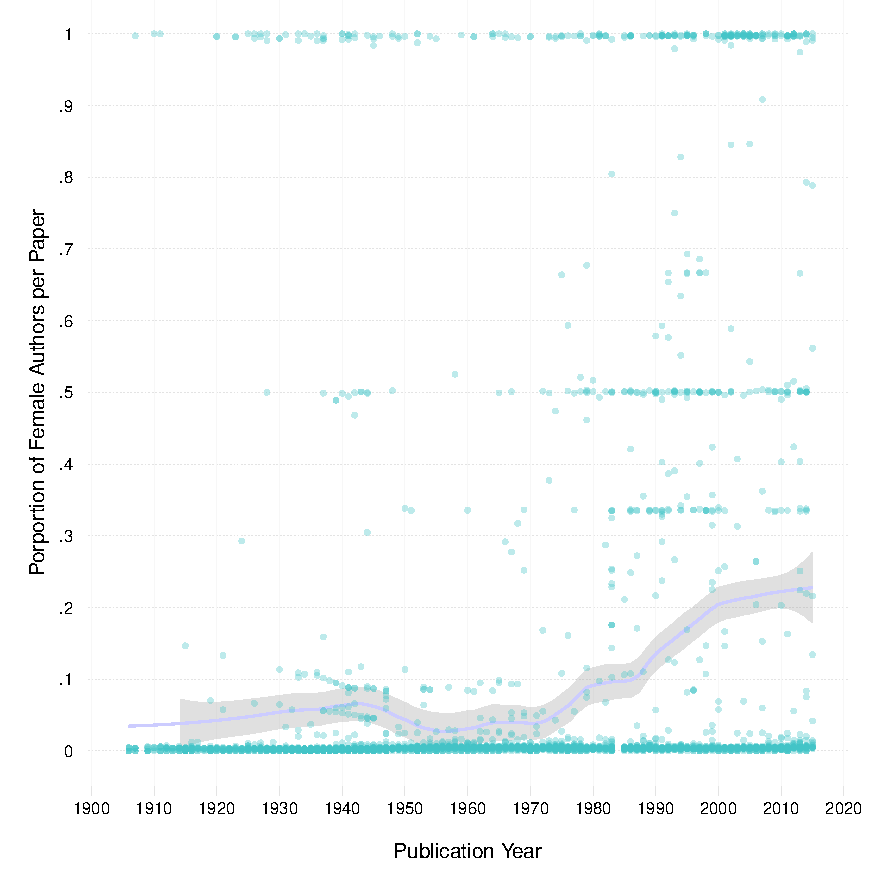
\includegraphics[scale=.85]{../figs/gender_authors_per_article_over_time.pdf}
\label{fig:women}
\end{figure}

\begin{figure}[htbp]
\centering
\caption{Abstract Views}
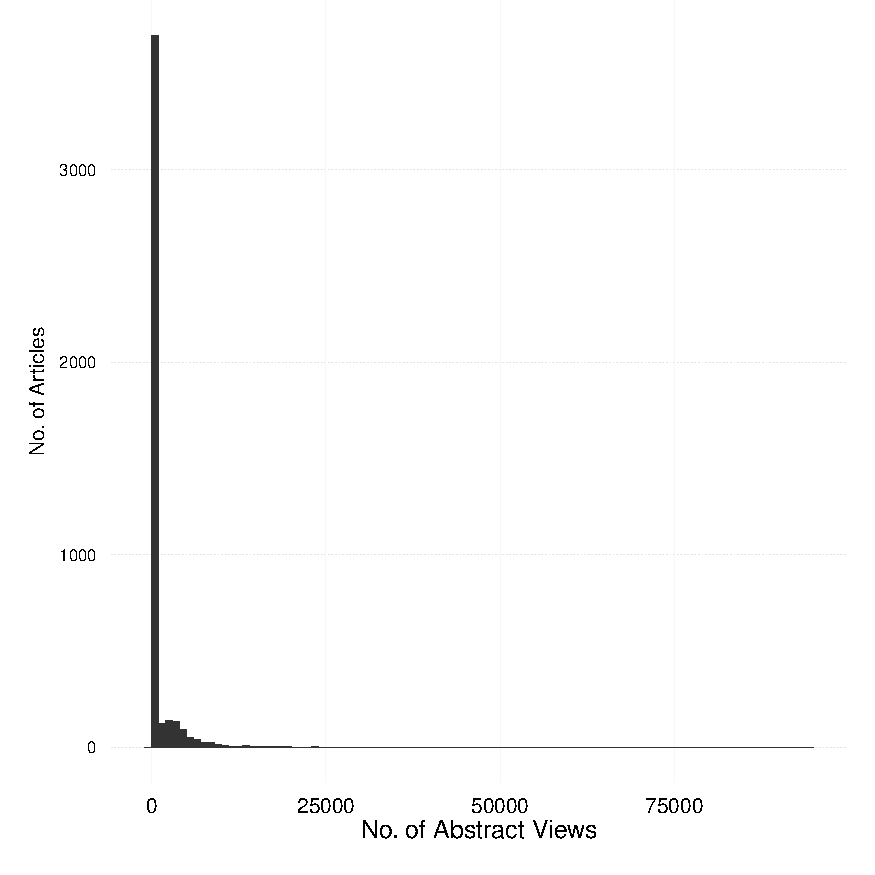
\includegraphics[scale=.85]{../figs/abstract_views.pdf}
\label{fig:abstracts}
\end{figure}

\begin{figure}[htbp]
\centering
\caption{Full-Text Views}
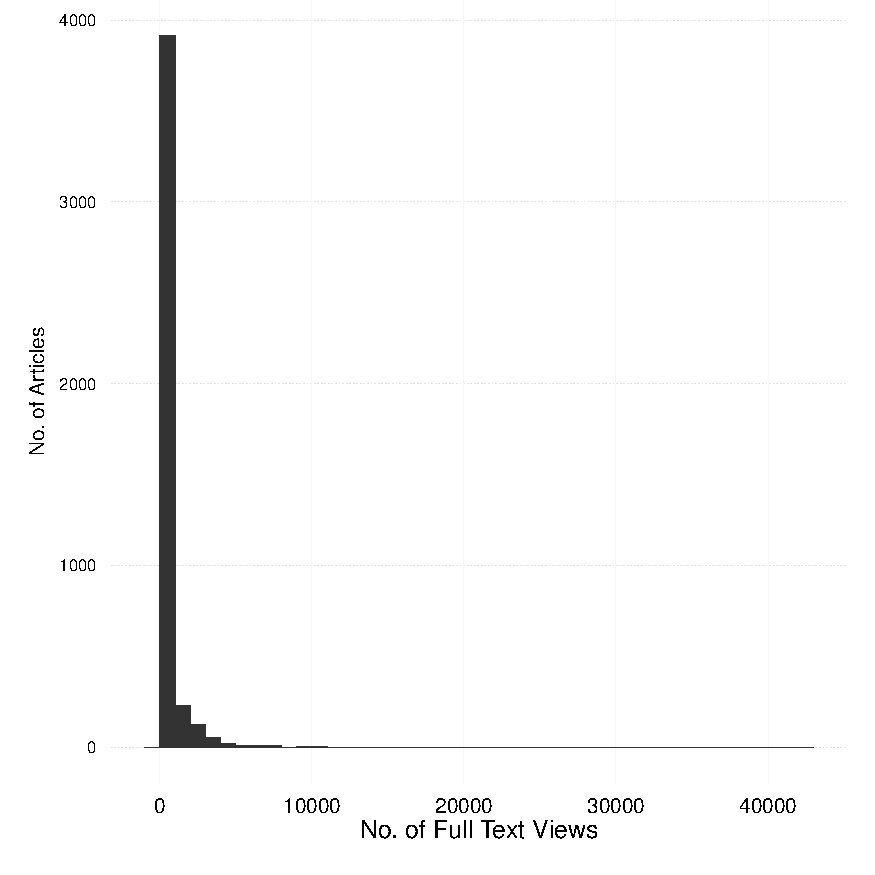
\includegraphics[scale=.85]{../figs/fulltext_views.pdf}
\label{fig:fulltext}
\end{figure}

\begin{figure}[htbp]
\centering
\caption{Title Length Over Time}
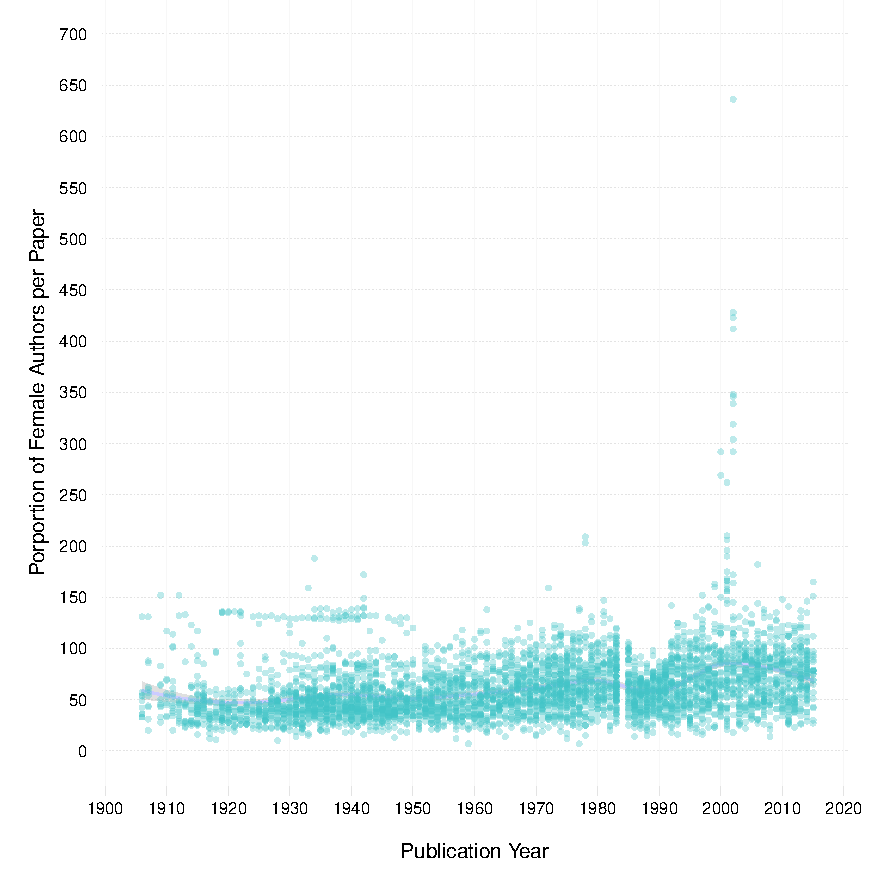
\includegraphics[scale=.85]{../figs/title_len_over_time.pdf}
\label{fig:fulltext}
\end{figure}

\clearpage
\bibliographystyle{apsr}
\bibliography{reviewbib}

\end{document}